% !TEX root=/home/tavant/these/manuscript/src/manuscript.tex




\chapter{Particle-In-Cell simulations of Hall Effect Thrusters}

Structure :

{\bf Particle in Cell simulations} 20 pages
\begin{zzz}
  1.1 Elements of the 2D PIC-MCC simulations

  1.2 Simulating a 3D system with 2D plans : the {\bf $R-\theta$} and {\bf $Z-\theta$} cases presentations, hypotheses

  1.3 Modeling Dielectrics : Poisson equation and SEE

  1.4 {\it Fake} axial convection in {\bf $R-\theta$} simulations
\end{zzz}


The \ac{HET} has been studied since its first designs int he 1960's.
However, the physical processes the govern its behaviour stay ill-understood.
For most of them, as the electron cross field mobility or the plasma-surface interactions, kinetic informations are needed.

\paragraph{Kinetic informations}
Usually, we use "kinetic" in contrast to the "fluid" description of a fluid or plasma.
In the fluid descriptions, the density, mean velocity and temperature are used to describe the system.
However, the fluid is constituted of a myriad of particle.
We can describe the particles inside an elementary volume by their velocity distribution.
The three first moment moment of the distribution are actually the density (\nth{0} moment), the velocity (\nth{1} moment) and the temperature (\nth{2} moment).
Equations and simulations dealing with the velocity distribution of the particles are named kinetic.

\ac{PIC} - \ac{MCC} simulations are one of the two main ways to conduct kinetic simulations, with the Vlasov solver, also known as \ac{DK} simulations.
While the \ac{DK} simulations using an Eulerian description of the position and velocity space, \ac{PIC} simulations uses an Lagrangian approach.

The next section present the basics of the \ac{PIC} - \ac{MCC} simulations, and the simulations code \LPPic that is develop at \ac{LPP}.

% !TEX root=/home/tavant/these/manuscript/src/manuscript.tex


\subsection{The Hall effect Thruster }
\label{sec-HET}

The \ac{HET} is an electrostatic electrical propulsion system accelerating ions by the mean of an imposed voltage difference.
\Cref{fig-bhtonoff} shows a picture of an \ac{HET} switch on and off.
We can clearly see the plasma in the annular chamber.


\begin{figure}[hbtp]
  \centering
  \includegraphics[width=\defaultwidth]{PPS-ON_OFF.jpg}
  \caption{Front view off an \ac{HET}, the BHT-1500 from Busek, USA}
  \label{fig-bhtonoff}
\end{figure}

We can summarize the composition of an \ac{HET} with four parts:
\begin{enumerate}
  \item The annular chamber.
  \item The injecting anode
  \item The cathode
  \item The magnetic circuit
\end{enumerate}

\begin{figure}[hbtp]
  \centering
  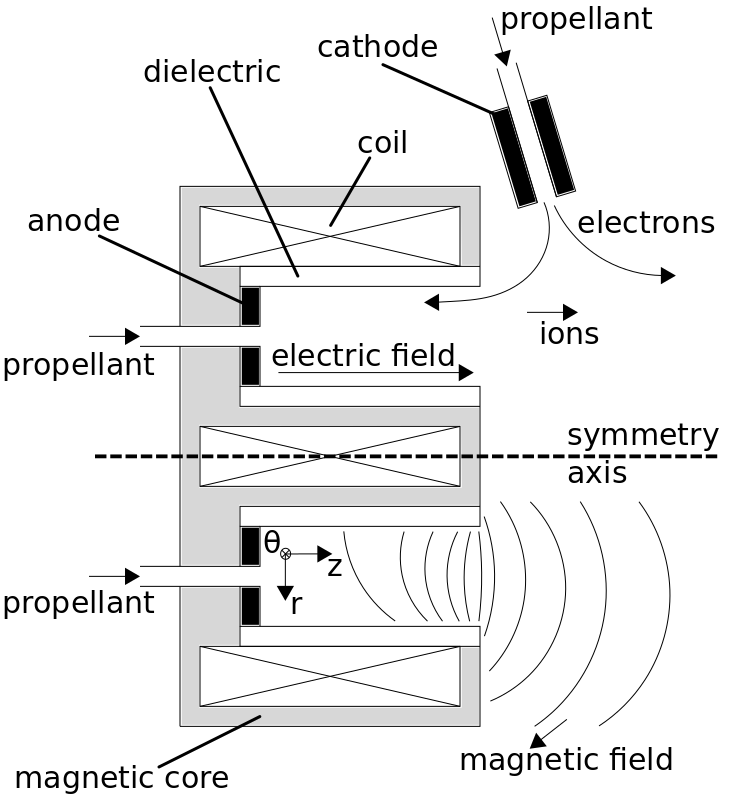
\includegraphics[width=\defaultwidth]{shematic_HET}
  \caption{Schematic cut of an \ac{HET}, illustrating its different parts. }
  \label{fig-shematiccut}
\end{figure}

\Cref{fig-shematiccut} presents a schematic cut of the \ac{HET} along its axial and radial direction.

\paragraph{The chamber} has an annular shape.
It is open closed at the anode side, and kept open at the other side.
The walls are usually constituted by a ceramic, usually \ac{BNSiO2}.
The material needs to be resistant to erosion by ion impact sputtering.
But changing the material is also known to affects the discharge behaviour.
The usually supposed phenomena for this impact is the secondary electron emission yield that is a function of the material nature.


\paragraph{The anode} is at the bottom of the chamber.
The anode voltage is imposed to a few hundred volts.
Usually, the neutral gas injection is made by the anode itself for
The mass flow rate is of the order of a flew mg/s.

\paragraph{The cathode} is outside of the chamber.
It is grounded, and injects electrons for two reasons:
\begin{itemize}
  \item most of the electrons ($\sim 90 \%$) are used to neutralize the ion flux, for both allowing the ions to leave the thruster and avoid charging of the spacecraft.
  \item some of the electrons are attracted by the anode, hence entering the chamber and allowing the plasma discharge and switch and remain on.
\end{itemize}

\paragraph{The magnetic circuit} is composed of electromagnets and a magnetic circuit mode of ferromagnetic material.
It create a constant radial magnetic field in the annular chamber.
The maximum value of the radial magnetic field is located close to the exit plan of the chamber.
Its amplitude is on the order of $200$ Gauss ($\sn{2}{-2}$ T).

\Cref{fig-bshape} illustrate the axial profile of the amplitude of the radial magnetic field.
\begin{figure}[hbtp]
  \centering
  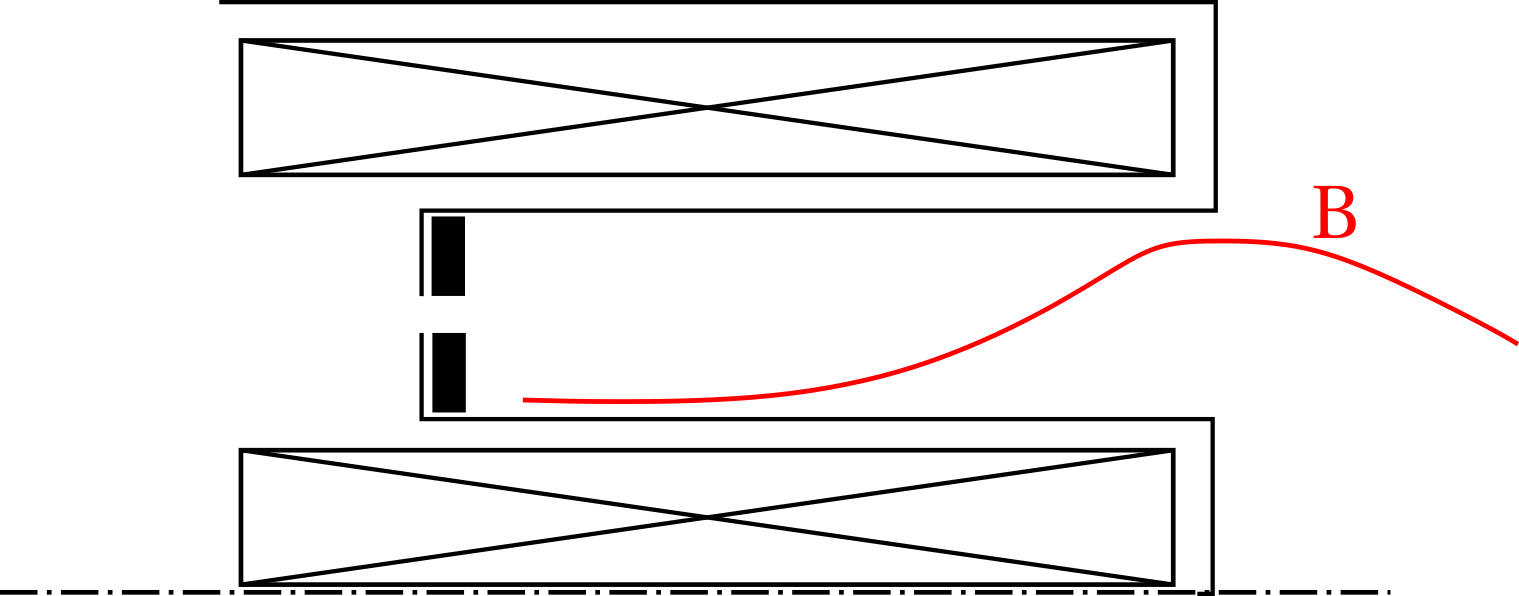
\includegraphics[width=\defaultwidth]{bshape}
  \caption{Usual shape of the axial profile of the radial magnetic field on the centreline of the channel.}
  \label{fig-bshape}
\end{figure}


\subsection{Operating principle}

The operation principle of an \ac{HET} is rather simple.
The objective is to ionize the propellant and impose an electric field to accelerate the ions.

\paragraph{Ionization}
Due to the low pressure (around $\sn{1}{-4}$ Pa), the mean free path of the electrons is too large, compared to the chamber size.
In consequence, we impose the magnetic field in order to trap the electrons in a cyclotron motion, increasing the residence time of the electron, and the ionization.
In average, 90\% of the propellant is ionized in an well designed \ac{HET}.

\paragraph{Acceleration}
The potential difference  between the anode and the cathode is used to accelerate the ions outside of the chamber and create the thrust.
Because the magnetic field slows the electrons down, the plasma resistivity increases in the region where the magnetic field amplitude is large.
Hence, the axial profile of the amplitude of the axial electric field presents a maximum close to the maximum of the magnetic field.

\paragraph{Ionization and Acceleration regions overlay}
As both the ionization region and the acceleration region are governed by the magnetic field, it can be difficult to obtain a net separation.
However, if ionization append in the acceleration region, the newly created ions will not be accelerated at their maximum velocity, hence resulting in a loss compared to the maximum theoretical thrust.

\Cref{fig-zones} shows an illustration of the amplitude of the ionization and the acceleration due tot he electric field.
\begin{figure}[hbtp]
  \centering
  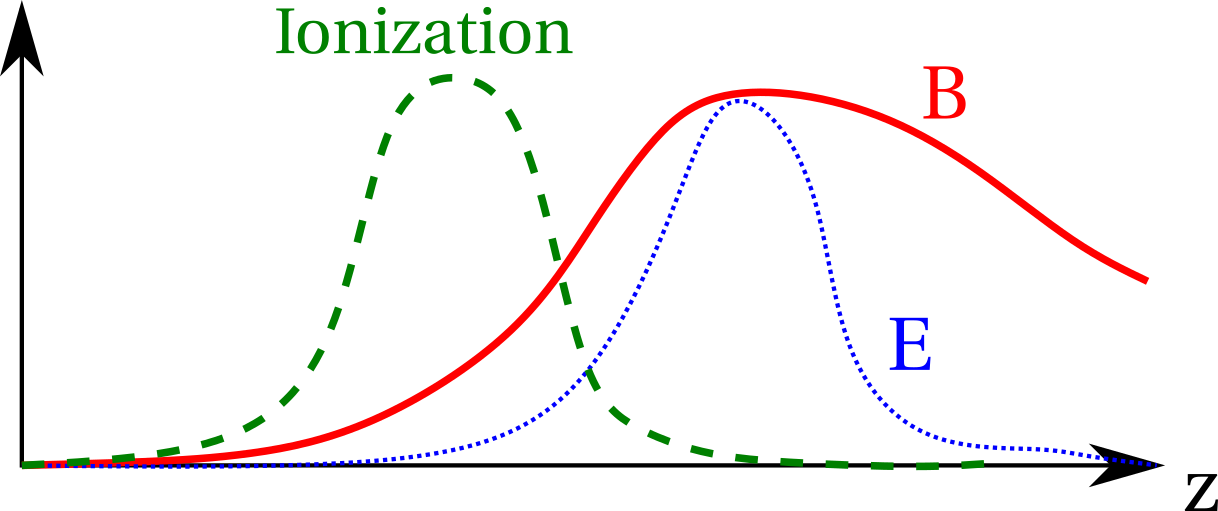
\includegraphics[width=\defaultwidth]{zones}
  \caption{Illustration of the usual axial profiles of the ionization and acceleration amplitude compared to the magnetic field.}
  \label{fig-zones}
\end{figure}

The thruster efficiency, in the usual configuration, is governed by its magnetic field topology.
Hence, it can be difficult to find the best topology that will optimize the ionization and the location of the regions.

Some concepts of double stage \ac{HET} have been proposed to decouple the two phenomena in order to control them independently.
However, the preliminary results are not as satisfactory as expected.
Moreover, the double-stage system needs more parts and power sources, resulting in a more complicated system.
Hence, we keep studying the usual single-stage configuration.

\subsection{Electron Drift and azimuthal instability}
The axial electric field $E$ and the radial magnetic field $B$ induces an azimuthal $E\times B$ drift of the electrons.
Because the ions are not significantly affected by the magnetic field, they do not drift.

As a consequence, they is a strong drift of the electron in respect  to the ions.
This drift can lead to instability in the azimuthal directions.
Because the drift is perpendicular to the magnetic field, it is usually called \ac{ECDI}.
However, as it rises from an $E\times B$ drift, some authors uses the name \ac{EDI}.

Azimuthal oscillations have been observed both experimentally and in simulations.
However, as the \ac{ECDI} characteristic are very close to usual \ac{IAW}, the community is still arguing about the actual kind of wave observed.


\subsection{Plasma-wall interaction}
The ceramic wall closes the chamber in the radial directions.
As usually observed in bounded plasmas, a floating plasmas sheath forms between the plasma and the dielectric wall.
The sheath confines the electrons in the plasma and accelerates the ions toward the walls.
This allows to obtain a flux of electron equals to the flux of ion, resulting in a charge conservation in the plasma, and a neutral flux, also named zero-net current to the surfaces.

Due to the relatively high electron energy, the material can emit electrons induced by electron impact.
These secondary electrons are accelerated toward the plasma, and so modify the plasma and the sheath properties.
The probability of \ac{SEE} depends of the electron impact characteristics (energy, angle) but also of the material: some material are more emitting than others.


\subsection{Cross field transport of the elections}
The electrons are not only drifting in the azimuthal directions.
For instance, because of collisions, the electrons can move from one magnetic line to another.
This leads to a cross-field transport in the direction of the electric field.

It has been observed in \ac{HET} that the electron cross-field transport is higher than the one only due to collisions.
Recently, the \ac{ECDI} has been proposed to induce this so-called anomalous transport of the electrons.

Another phenomena that can leads to increased cross-field transport in the \ac{NWC}.
It is due to electron collisions with the wall, inducing \ac{SEE}.


\section{Three-dimensional physics}
\label{sec-3Dphi}

The physics of the \ac{HET} is really three dimensional:

\begin{itemize}
  \item The plasma is accelerated in the axial direction. The axial profile of the magnetic field is responsible for the performance of the thruster.
  \item The radial dimension is closed by the chamber walls. The walls are responsible for most of the plasma losses, both on the particle and energy balances.
  \item The electrons drifts in the azimuthal direction, leading to instabilities.
\end{itemize}

Consequently, when simulating an \ac{HET}, if one of the direction is not model, a part of the physics will be missing:
\begin{itemize}
  \item Missing axial direction: the ionization and the convection are missing
  \item Missing radial direction: the wall losses and interactions are missing
  \item Missing azimuthal direction: the \ac{ECDI} is missing, hence the electron cross-field transport is not well represented.
\end{itemize}

While 3D-simulations have recently been proposed, they uses scaling laws to simulate the system in a reasonable amount of time.
A simulation at scale {1:1} is not yet accessible.
Hence, we need to rely on \ac{1D} or \ac{2D} simulations.
Consequently, we need to take into account the missing physics or include a model of its effects on the system.

% % !TEX root=/home/tavant/these/manuscript/src/manuscript.tex

\section{Elements of the 2D PIC-MCC simulations}
  \label{sec-elements}
  \subsection{Principe of the PIC simulations}

    The \ac{PIC} simulation models particles moving freely on a grid.
    The grid is used to compute the electric field, in the electrostatic approximation by solving the Poisson equation

    \begin{equation}
      \label{eq-poisson}
      \Delta \phi = - \frac{\rho}{\epsilon_0}
    \end{equation}

    where $\phi$ is the electric potential, $\rho$ is the charge density, and $\epsilon_0$ the vacuum permittivity.
    If the electrostatic approximation is not correct, one needs to solve the Maxwell equations.

    The particles move following the Lorenz forces
    \begin{equation}
      \label{eq-Lor}
      m \vec{a} = q \vect{E} + q \vec{v} \times \vec{B}
    \end{equation}
    with $m$ and $q$, the particle mass and electric charge, respectively.
    The numerical particles followed in the simulations correspond to $q_f$ physical particles, with
    \begin{equation}
      q_f = \frac{n V}{\Npc}
    \end{equation}
    with $n$ the particle density, $V$ the volume of a cell, and $\Npc$ the number of numerical particles in a cell.
    A large enough number of particles is needed in order to obtain physical results.
    Indeed, an insufficient number of particles leads to numerical heating \cite{ueda1994}.
    Usually, a minimum of 100 particles per cell are used, but recent results seem to encourage to use more particles \cite{janhunen2018}.

  \subsection{Monte Carlo collisions}

    In \ac{PIC} simulations, collisions between charged and neutral particles can be modeled by binary collision, but this approach is computationally costly.
    Instead, a Monte-Carlo algorithm can be used \cite{vahedi1995}.
    This approach is very efficient and allows scattering, momentum transfer, and ionization to be consistently modeled.
    The propellant used in \ac{HET} is \ac{Xe}.
    The cross-sections used for modeling \ac{Xe} or other gases collisions are taken from the {\sc LXCat} database project \cite{LXCat_web,pancheshnyi2012}.
    Except if otherwise stated, the elastic, inelastic scattering and ionization reactions listed in \cref{tab-reactXe} are used.
    The cross-section values are summarised in \cref{fig-xexsection}.

    \begin{table}[hbtp]
      \ra{1.3}
      \centering
      \caption{Reactions for xenon used in the PIC simulations}
      \label{tab-reactXe}
      \begin{tabular}{@{}lll@{}}  \toprule
        Reaction & Threshold & Reference\\ \midrule
        {\it Elastic scattering} & &\\
        e + Xe = e + Xe   & --   & \cite{Lxcat_Xe,Lxcat_Xe2} \\
        {\it Excitation} & &\\
        e + Xe = e + Xe$^*$   & 8.315eV   & \cite{Lxcat_Xe,Lxcat_Xe2} \\
        e + Xe = e + Xe$^*$   & 9.447eV   & \cite{Lxcat_Xe,Lxcat_Xe2} \\
        e + Xe = e + Xe$^*$   & 9.917eV   & \cite{Lxcat_Xe,Lxcat_Xe2} \\
        e + Xe = e + Xe$^*$   & 11.7eV    & \cite{Lxcat_Xe,Lxcat_Xe2} \\
        {\it Ionization} & &\\
        e + Xe = e + Xe$^+$   & 12.13eV   & \cite{Lxcat_Xe,Lxcat_Xe2} \\
        \bottomrule
      \end{tabular}
    \end{table}



    \begin{figure}[hbtp]
      \centering
      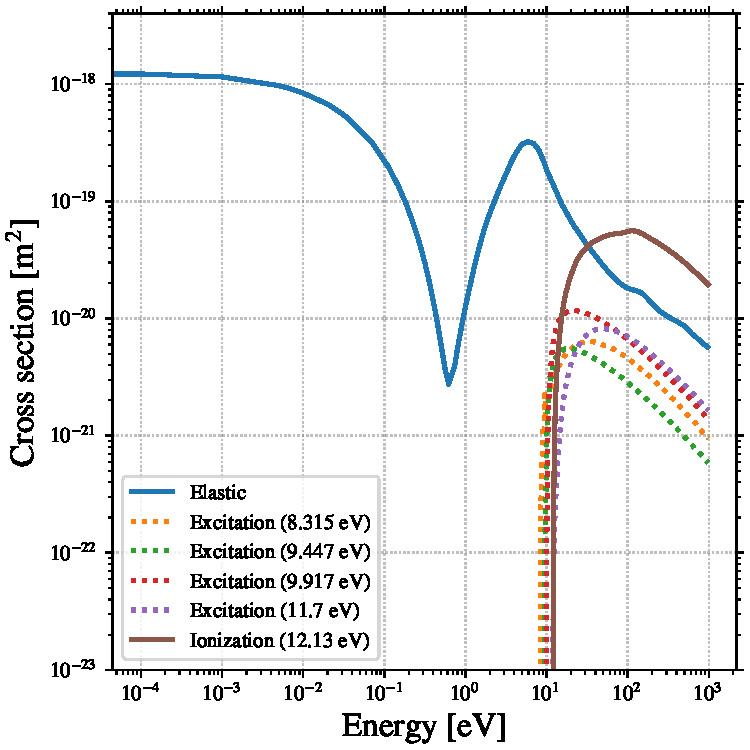
\includegraphics[width=\defaultwidth]{figure/xenon_cross_section.pdf}
      \caption{Cross section values used in the Monte Carlo procedure \cite{Lxcat_Xe,Lxcat_Xe2}.}
      \label{fig-xexsection}
    \end{figure}


\section{Numerical implementation of the Particle in cell simulation}

  \LPPic is an explicit electrostatic \ac{PIC}-\ac{MCC} simulation code.
  Every time-step, the simulation loop presented in \cref{fig-picloop} is computed.
  The different steps constituting the PIC-loop are described in the next subsections.
  \begin{figure}[hbtp]
    \centering
    \smartdiagramset{circular distance=4.5cm,
    module minimum width=3.5cm,
    text width=3cm,
    arrow tip=to}
    \smartdiagram[circular diagram:clockwise]{Particle Motion ,Boundary,Collision,Density weighting, Poisson Equation, Field weighting}
    \caption{\ac{PIC}-\ac{MCC} loop executed every time step.}
    \label{fig-picloop}
  \end{figure}


  \subsection{Data used}
    In \ac{PIC} simulations, there are two kinds of data used\string:
    \begin{itemize}
      \item Particles (electrons, ions, neutrals can be followed as well but not in \LPPic)
      \item Mesh, also named fields (densities, electric and magnetic fields, and so on)
    \end{itemize}

    \paragraph{Particles\\}
    For each particle, are known its position $\vec{x}$ and its velocity $\vec{v}$.
    In most \ac{PIC}-\ac{MCC} simulations, the three directions of the velocity vector are followed in order to take into account scattering.
    It is abbreviated as \acs{3V}.
    The particle positions and velocity are not discretized, except to the numerical floating-point precision.

    \paragraph{Fields\\}
    The fields are defined at the center of each cell of the mesh.
    The charge density $\rho$ is computed by depositing the particle on the mesh, using the Cloud-in-cell model \cite{birdsall1991}.
    The electric field at the position of the particle is also obtained by bilinear interpolation.
    The mesh dimension defines the dimension of the simulation.
    It is usual to find \acs{1D}\acs{3V} or \acs{2D}\acs{3V} \ac{PIC} simulations, for particles with 3 directions on the velocity but one (or two) dimensions in space.

    \subsection{Particle pusher}
    The interaction of the movement equation \cref{eq-Lor} is different for magnetized and non-magnetized particles.
    For non-magnetized particles, we use the leapfrog scheme \cite{birdsall1991}
    \begin{align}\label{eq-leapfrog}
      \vect{v}^t &= \vect{v}^{t-1} + \frac{q}{m} \vect{E} \dt, \\
      \vect{x}^t &= \vect{x}^{t-1} + \vect{v}^t \dt,
    \end{align}
    with the superscript $t$ designing the time step, $q$ and $m$ the particle electric charge and mass, $\vect{E}$ the electric field at the particle position, and \dt the time step duration.

    It is important to note that the leapfrog induces a shift of $\frac{\dt}{2}$ between the position and the velocity, as illustrated in \cref{fig-leapfrog}.
    \begin{figure}[hbtp]
      \centering
      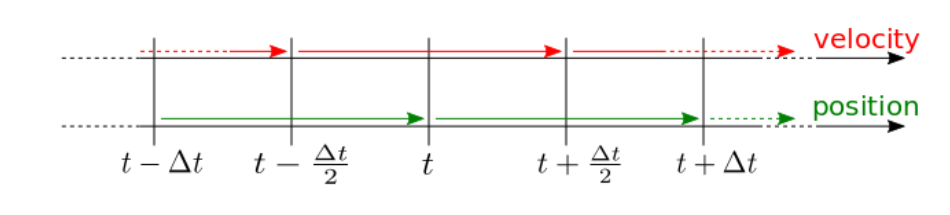
\includegraphics[width=\defaultwidth]{leapfrog.png}
      \caption{Illustration of the shift between the particle velocity and position.}
      \label{fig-leapfrog}
    \end{figure}
    This shift can lead to erroneous diagnostics when computing moments of the particles distribution.
    For instance, the mean velocity of an ensemble of $N$ particles at the instant $t$ is computed as\string:
    \begin{equation} \label{eq-meanv}
      \mean{\vect{v}}^t = \frac{1}{N} \sum_i^N \lp \vect{v_i}^t + \frac{q}{m} \vect{E_i} \frac{\dt}{2} \rp.
    \end{equation}
    Other moments like the mean energy or heat flux follow the same correction.
    We can see that the error between $\mean{\vect{v}}$ defined above and
    $$ \tilde{\vect{v}} = \frac{1}{N} \sum_i^N  \vect{v_i}^t $$
    is
    $$ \mean{\vect{v}} - \tilde{\vect{v}} =\frac{q \dt}{2 m}  \frac{1}{N}  \sum_i^N  \vect{E_i} .$$
    Hence, the error in the diagnostic is larger in the region of large electric field (as in the sheaths).

    \paragraph{Magnetized particles}
    For magnetized particles, we use a modification of the leapfrog algorithm proposed by Boris \cite{boris1970}.
    It corresponds to an operator splitting between the electrostatic acceleration and the magnetic rotation.
    This splitting is described below\string:

    \begin{enumerate}
      \item accelerate the particle during $\frac{\dt}{2}$\string: $\vect{v}^{t-\frac{\dt}{2}} = \vect{v}^{t-1} + \frac{q}{m} \vect{E} \frac{\dt}{2}$
      \item rotate the particle velocity with the magnetic field
      \item accelerate the particle during $\frac{\dt}{2}$\string: $\vect{v}^t = \vect{v}^{t-\frac{\dt}{2}} + \frac{q}{m} \vect{E} \frac{\dt}{2}$
    \end{enumerate}


  \subsection{Poisson equation solver}
  \label{subsec-poissonintro}

    In order to compute the electric field due to the particle charge density, the Poisson equation \cref{eq-poisson}  needs to be discretized over the mesh.
    We can directly discretize the differential operator by using the finite volume approach over a cell of the mesh.
    The formal discretization is developed in \cref{sec-diel}, for the particular case of taking into account the presence of dielectric boundaries.

    In \ac{1D}, the obtained linear system is tridiagonal.
    It can be solved directly using {\sc Thomas}' algorithm, which stores the Gauss elimination's coefficient.
    In \ac{2D}, the linear system is pentadiagonal.
    A direct solver, like the $LU$ decomposition, would require a large amount of memory to store the factorization matrices.
    On the other hand, as the time step is usually small in \ac{PIC} simulation, we expect the plasma potential $\phi$ not to change rapidly.
    Hence, an iterative solver using the previous solution as an initial guess seems more reasonable from both the memory storage and the computational time.
    
    \inlinenote{Anne: dire ici dans quelle section, tu vas en reparler}
    

    
% !TEX root=/home/tavant/these/manuscript/src/manuscript.tex

\section{Bidimentionnal simulation of an \ac{HET}}

We are interested in studying the azimuthal instabilities and the induced electron transport in the axial direction.
In addition, we want to study the plasma-wall interactions.
As realistic \ac{3D} simulations are not yet achievable, we choose to simulate the radial-azimuthal plan.
The axial location where the electron drift is the highest is close to the exit plan, where the axial electric field is the highest.
Hence, we choose this location to be simulated.
In this section, we describe the characteristics of the radial-azimuthal simulation.


\subsection{Neglecting curvature}
The \ac{ECDI} features oscillations of short wavelength of the order of the mm.
Hence, neglecting the curvature of the channel is expected not the change the \ac{ECDI} characteristics while improving the simulation performances.

In  \citet{heron2013},  the authors have performed a \ac{2D} \ac{PIC} simulation including the channel curvature.
They have observed a small difference between the inner and the outer walls.
In  \citet{dominguez-vazquez2018}, the authors studied the effect of the curvature using a \ac{1D} radial model.
They have shown asymmetries due to the combination of the geometric expansion, the magnetic mirror effect, and the centrifugal force.
However, the global behavior of the discharge is not affected compared to simulations without the curvature model.
Hence, in order to simplify the analogy, we choose to neglect the curvature.

Consequently, we can use a Cartesian mesh (also called a rectangular mesh).
The usual notation $x,y$ is used in the simulation for the radial ($r$) and azimuthal directions $\theta$, respectively.
The $z$ component corresponds to the axial direction, normal to the simulation domain.

\subsection{Radial-azimuthal domain description}

The azimuthal direction is closed using a periodic boundary condition for both the particles and the fields.
The radial direction is closed by walls.
The walls can be grounded metallic, or a dielectric boundary can be model.
They are described and discussed in \cref{sec-diel}.

A constant and uniform magnetic field $B_0$ is imposed in the radial direction.
This does not take into account the magnetic mirror, that has been shown to be important \citep{keidar2005,yu2008a,dominguez-vazquez2018}.
However, it cannot be modeled in the \ac{2D} Cartesian radial-azimuthal domain while conserving a divergent-free magnetic field topology.
A constant and uniform axial electric field $E_0$ is imposed.
\Cref{fig-2dschemat} shows a schematic representation of the simulated domain, overlaid with the computed azimuthal electric field $E_y$.

\begin{figure}[hbtp]
  \centering
  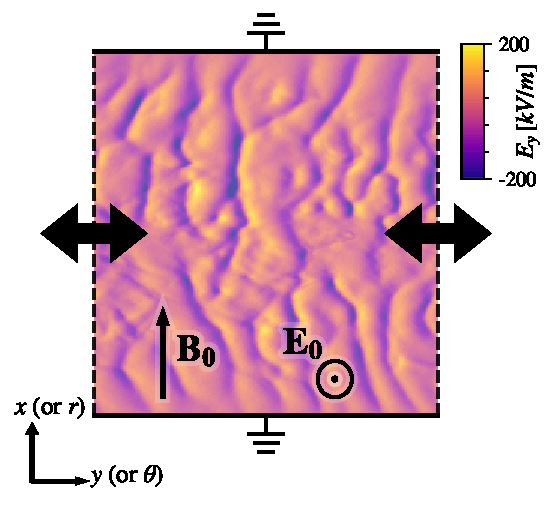
\includegraphics[width=\defaultwidth]{2D_schema.pdf}
  \caption{Schematic representation of the radial-azimuthal simulation domain. Overlaid is the computed azimuthal electric field given as an example. The radial dimensions lengths 2\,cm, and the azimuthal length is 1\,cm.
  The magnetic field is $B_0=0.02\,\tesla$, the axial electric field is $E_0=\sn{2}{4}\,\volt\per\meter$, and the walls are grounded. More parameters are given in \cref{parameters}.}
  \label{fig-2dschemat}
\end{figure}

\subsection{Particle balance}
As the axial position simulated is the exit plane, the ionization is too low to balance the particle losses to the wall.
Instead, the ionization takes place upstream, and the particles are convected downstream.
In these conditions, two models can be used concerning the particle losses at the walls\string:
\begin{itemize}
  \item having a simulation that dies off, as done in \citet{janhunen2018},
  \item forcing an arbitrary ionization to occur in order to compensate the radial losses \citep{dominguez-vazquez2018}.
\end{itemize}
The second option is slightly less realistic, but allows to obtain a steady-state and is supposed not to affect the simulation significantly.
Hence, we use this model to achieve a constant mean plasma density during the simulation.
The forced ionization rate is computed in order to compensate the losses of the ions at each time step.
The spacial ionization  profile is uniform.


\subsection{Axial convection}

Due to the imposed axial electric field, ions and electrons gain energy.
In the \ac{HET}, the axial convection of the particles balances the energy gain.
However, in a purely \ac{2D} simulations, the convection is missing, resulting in an ever-rising particle energy.
This prevents the possibility to reach a steady-state regime, as observed in \citet{heron2013,janhunen2018}.

We implemented a model of convection initially proposed for a \ac{1D} simulation by \citet{lafleur2016a}, and adapted in \ac{2D} by \citet{croes2017a}.
The model uses a finite axial length $L_z$.
When a particle reaches the boundary $z=0$ or $z=L_z$, it is removed from the simulation.
In order to conserve the particle (and charge) balance, a particle is created at $z=0$ for the ions (that are accelerated toward $z>0$) or at $z=L_z$ for the electrons.
It has been observed that using a radial position chosen uniformly at random for the newly injected particle would affect the sheath \citep{croes2017a}.
Hence, the radial position of the new particle is the same as the removed particle.

Concerning the azimuthal particle position, it is more difficult to choose between a random position or the same position as the removed particle.
In \citet{lafleur2016a,croes2017a}, a random azimuthal position was chosen.
However, as will be discussed in \cref{sec-reinjectionnoise}, this induces a numerical noise that can be harmful in some cases.

% !TEX root=/home/tavant/these/manuscript/src/manuscript.tex

\section{Dielectrics boundary condition}
  \label{sec-diel}

  \Cref{fig-2dschemat} shows the simulation of the radial-azimuthal domain with metallic grounded walls.
  \Cref{fig-2D} illustrates the configuration in the radial-azimuthal plane highlighting the more realistic radial boundary conditions.
  The plasma is bounded in the radial direction by dielectric layers isolating the magnetic circuit.
  The magnetic circuit can be considered electrically grounded.

  The particles are absorbed when touching the dielectric wall, and we suppose an infinite residence time.
  Hence, we obtain a surface charge $\sigma$ at a time $t$ with
  \begin{equation} \label{eq-sigmaintegrate}
    \sigma(t) = e \int_0^t (J_i - J_e) dt
  \end{equation}
  with $J_i$ and $J_e$ the ion and electron flux respectively and $e$ is the elementary charge and supposing that there is no surface charge at the interface at the beginning.

  \begin{figure}[hbt]
    \centering
    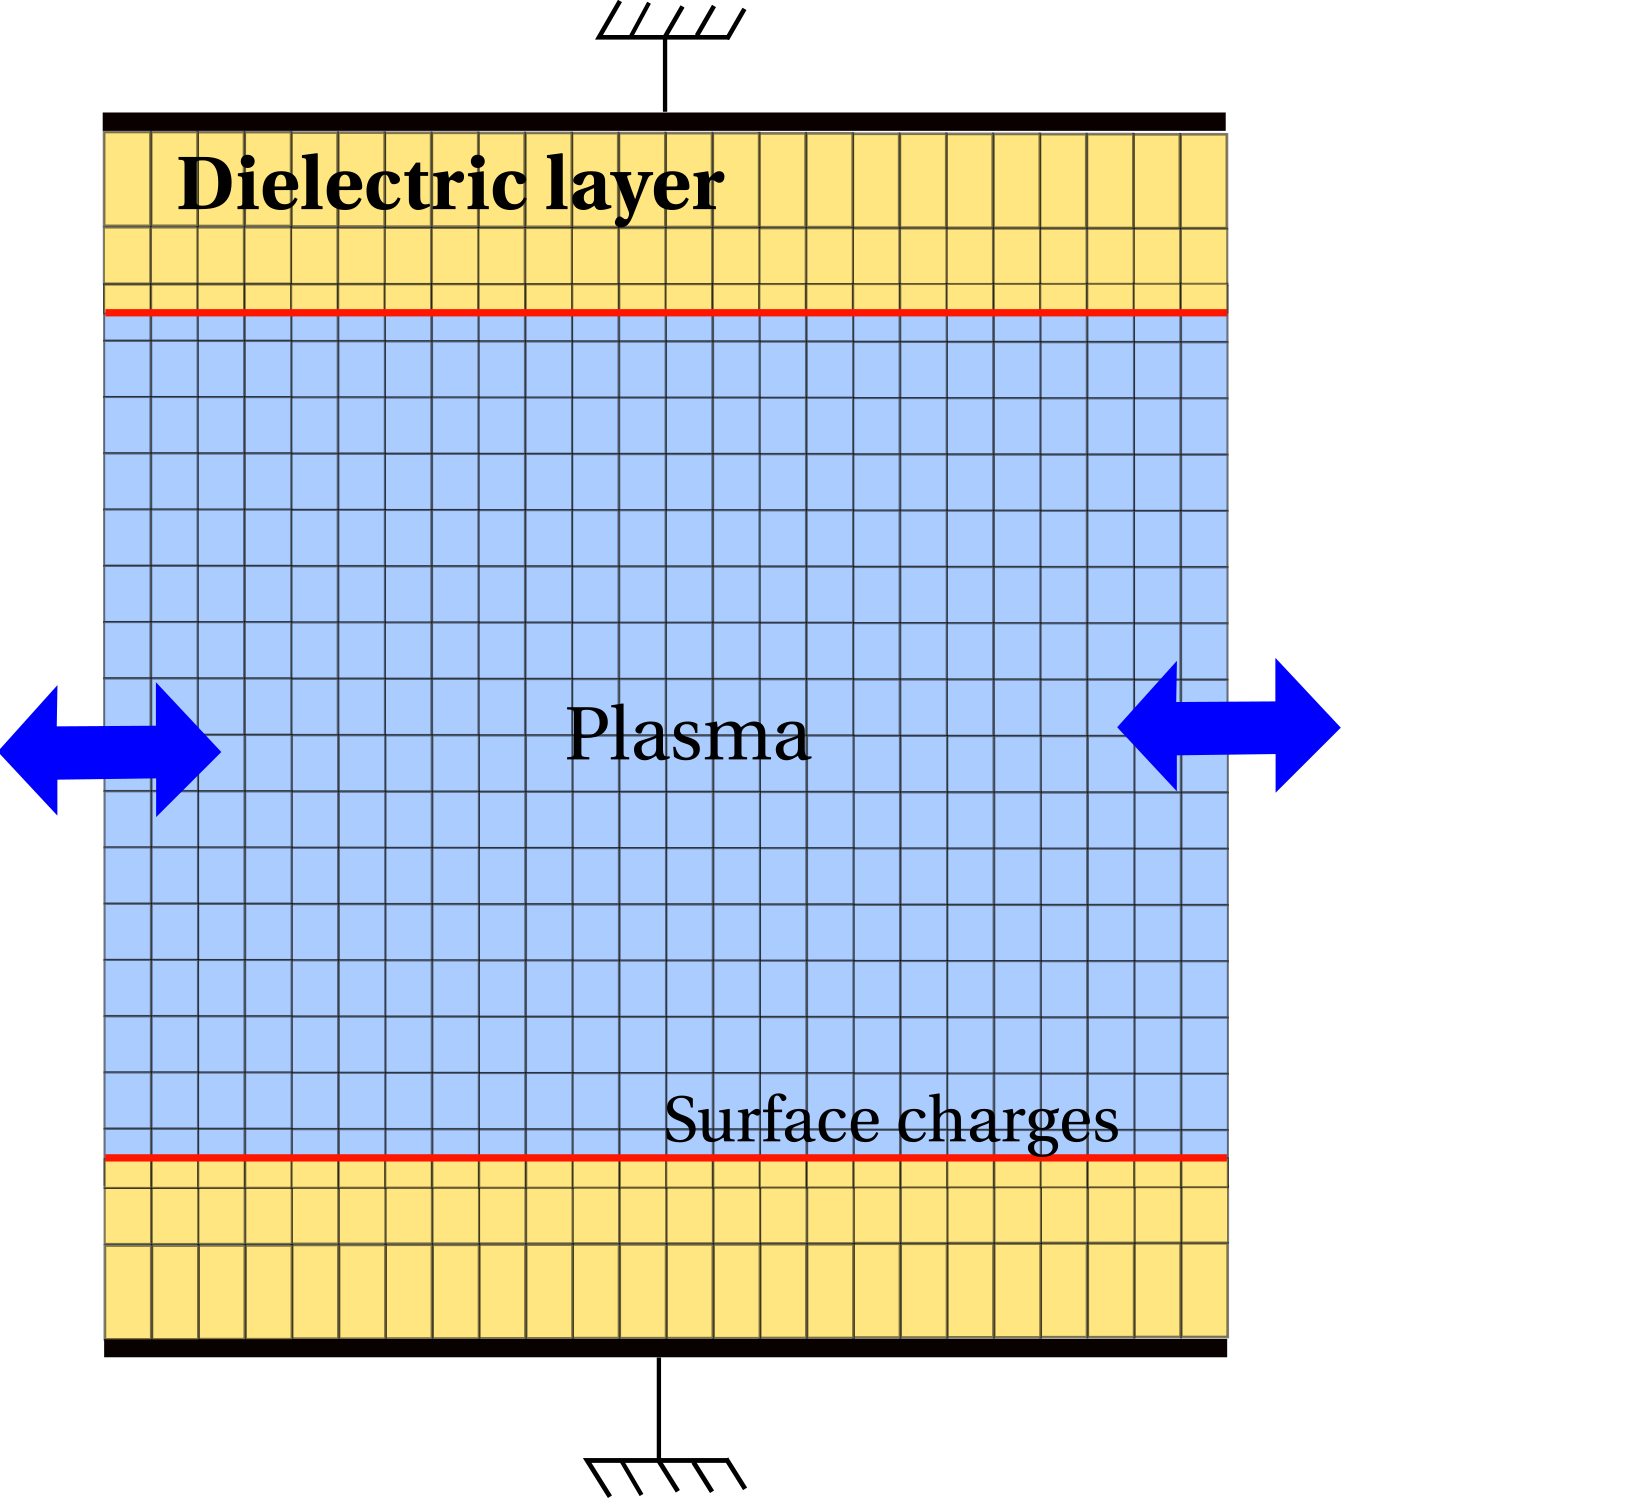
\includegraphics[width=\defaultwidth]{2D_diel_Rtheta}
    \caption{Schematic representation of the dielectric layers between the plasma in the \acs{2D} radial-azimuthal plane. Are present the dielectric in yellow, the plasma in blue, the surface charges in red, and the grounded magnetic circuit in black.}
    \label{fig-2D}
  \end{figure}


  A common approach is to assume that the electric field inside the dielectric is zero \citep{taccogna2019}. 
  Using Gauss theorem, we obtain a Neumann boundary condition at the plasma-wall interface for the potential
  \begin{equation} \label{eq-gauss}
    \norm{\partial_r \phi} = \frac{\norm{\sigma}}{\epsilon_0}
  \end{equation}
  with $\sigma$ the surface charge and $\epsilon_0$ the vacuum permittivity.
  However, the electric field in a dielectric material is not zero but depends on the global system.
  Hence, in order to model the dielectric wall of the \ac{HET} correctly, we choose to include the whole dielectric layers inside of the simulation domain.

  In this section, we derive the discretization of the Poisson equation with a non-uniform permittivity in the \ac{2D} radial azimuthal plane using the finite volume approach.


  \subsection{Non-uniform mesh}

    In the dielectric layers, there is no particle nor charge.
    Hence, the numerical constraints on the cell size are not applicable, and the cell size can be increased.
    In order to reduce the cell size difference between two neighboring cells, we use an exponential growth of the cell size in the radial direction.
    The cell size in the azimuthal direction $\dy$ is kept constant.
    The resulting non-uniform mesh can be seen in \cref{fig-2D}.


  \subsection{Poisson equation discretization}


  The dielectric permittivity is $\epsilon= \epsr \epsilon_0$ with $\epsr$ the relative permittivity of the dielectric.
  The Poisson equation with a not-constant permittivity is
  \begin{equation} \label{eq-poissondiel}
    \grad \cdot \epsilon \grad \phi = \rho
  \end{equation}
  with $\rho$ the charge density.
  We note $\vect{D}=\epsilon \vect{E} = \epsilon \grad \phi$ the electric flux.
  \Cref{fig-decompo1} shows the Cartesian decomposition of the \ac{2D} domain.
  The cell $(i,j)$ has four direct neighbors\string:
  \begin{itemize}
    \item the east $E$ in $(i+1,j)$
    \item the west $W$ in $(i-1, j)$
    \item the north $N$ in $(i, j+1)$
    \item the south $S$ in $(i, j-1)$
  \end{itemize}
  The cell dimensions are $\dx_{i,j}$ and $\dy_{i,j}$, and $\V=\dx_{i,j} \dy_{i,j}$ is the cell volume.
  As the mesh is Cartesian, we have for a given $j$ $\dx_{i,j} = cst$ for all $i$. Hence, we note $\dx_{i,j} = d_i$ and $\dy_{i,j} = d_j$

  The boundaries are noted $S^s_{i,j}$ with $s=E,W,N$ or $S$.
  We can see that $S^W_{i,j}=S^E_{i-1,j}$, and the same goes for the other borders.
  We note $\C = S^E_{i,j} \cup S^W_{i,j} \cup S^N_{i,j} \cup S^S_{i,j}$ the cell surface boundary.
  The center of the cell is located in $i,j$ and the borders are located in $i\pm 1/2$ in the East-West direction and $j\pm 1/2$ in the North-South direction.
  \begin{figure}[hbt]
    \centering
    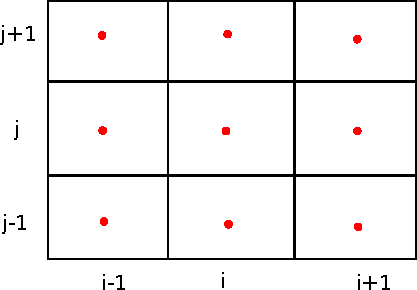
\includegraphics[width=\defaultwidth]{discrect1.pdf}
    \caption{Illustration of the Cartesian decomposition of the \acs{2D} domain}
    \label{fig-decompo1}
  \end{figure}


  \subsection{Poisson equation discretization}

    We start by positioning the plasma-dielectric interface on the surface between two cells.
    This means that the permittivity $\epsilon = \epsilon_0 \epsr$ is  constant over a cell.
    In order to discretize the Poisson equation, we integrate \cref{eq-poissondiel} over the cell volume

    \begin{equation}
    \int_{\V} - \grad \cdot (\epsilon \grad \phi) dv= \int_{\V} \rho dv.
    \end{equation}
    Using Gauss-Ostrogradsky theorem, we obtain
    \begin{equation}
    \oint_{\C} ( - \epsilon \grad \phi) \cdot \vect{n} dS = Q_{tot} =  \V \bar{\rho},
    \end{equation}
    with $\vect{n}$ the normal vector directed outward, $Q_{tot}$ is the total charge of the cell and $\bar{\rho}$ is the mean value of $\rho$ in the cell.
    We can decompose the integration over the cell boundary with the four surfaces $S^s_{i,j}$ as
    \begin{equation}
      \label{eq-poissonsum}
    \oint_{\C} (-\epsilon \grad \phi) \cdot \vect{n} dS = \sum_{k\in(E,W,N,S)} S^k_{i,j} \vect{D}^k_{i,j} \cdot \vect{n}
    \end{equation}
    with $\vect{D}^k_{i,j}$ the flux through the surface $k$ of the cell $(i,j)$.


    \paragraph*{Electric flux \\}
    Let us define the electric flux through the East border  $\vect{D}^E_{i,j}$.
    We suppose there is no surface charges on $S^E$.
    We can hence write the electric flux as
    \begin{align} \label{eq-flux1}
      \vect{D}^E_{i,j} \cdot \vect{n} &= \epsilon_{i,j} E_{x, i+1/2,j}^-\\
                                      &= - \epsilon_{i,j} \frac{\phi_{i+1/2,j} - \phi_{i,j}}{d_i/2},
    \end{align}
    with an off-center discretization of the electric field.
    Using the Gauss's law without charges
    \begin{equation} \label{eq-gausslaw}
      \epsilon_{i,j}E_{x, i+1/2,j}^- - \epsilon_{i+1,j}E_{x, i+1/2,j}^+ =0,
    \end{equation}
    we have
    \begin{equation}
      \epsilon_{i,j} \frac{\phi_{i+1/2,j} - \phi_{i,j}}{d_i/2} = \epsilon_{i+1,j} \frac{\phi_{i+1,j} - \phi_{i+1/2,j}}{d_{i+1}/2}.
    \end{equation}
    Hence
    \begin{equation} \label{eq-phidemi1}
      \phi_{i+1/2,j} = \frac{\epsilon_{i,j} d_{i+1} \phi_{i,j} + \epsilon_{i+1,j} d_{i} \phi_{i+1,j} }{\epsilon_{i,j} d_{i+1} + \epsilon_{i+1,j} d_{i} },
    \end{equation}
    which corresponds to the usual discretization \citep{croes2017} when $\epsilon$ and $d_i$ are both constant.
    Using \cref{eq-phidemi1} in \cref{eq-flux1} we obtain
    \begin{align}
      \label{eq-nosc}
    \vect{D}^E_{i,j} \cdot \vect{n} &=& 2\frac{\epsilon_{i,j}\epsilon_{i+1,j}}{\epsilon_{i,j}d_{i+1} + \epsilon_{i+1,j} d_i} (\phi_{i,j}-\phi_{i+1,j})
    &=& 2\epsilon_0 \frac{\epsr{i,j}\epsr{i+1,j}}{\epsr{i,j}d_{i+1} + \epsr{i+1,j} d_i} (\phi_{i,j}-\phi_{i+1,j})
    \end{align}

    We note $Q^E_{i,j} \equiv \frac{\epsilon_{i,j} \epsilon_{i+1,j}}{\epsilon_{i,j} d_{i+1} + \epsilon_{i+1,j} d_i}$.
    reproducing the same decomposition on the other borders, we obtain
    \begin{equation}
      \label{eq-descretPoisson1}
    S^E_{i,j} Q^E_{i,j} \phi_{i+1,j} + S^W_{i,j} Q^W_{i,j} \phi_{i-1,j} + S^N_{i,j} Q^N_{i,j} \phi_{i,j+1} + S^S_{i,j} Q^S_{i,j} \phi_{i,j-1} - Q^C_{i,j} \phi_{i,j} = - \V \bar{\rho_{i,j}}
    \end{equation}
    with
    \begin{center}
      $\begin{dcases}
     Q^E_{i,j} &= 2\frac{\epsilon_{i,j} \epsilon_{i+1,j}}{\epsilon_{i,j} d_{i+1} + \epsilon_{i+1,j} d_i} \\
     Q^W_{i,j} &= Q^E_{i-1,j} \\
     Q^N_{i,j} &= 2\frac{\epsilon_{i,j} \epsilon_{i,j+1}}{\epsilon_{i,j} d_{j+1} + \epsilon_{i,j+1} d_{j}}\\
     Q^S_{i,j} &= Q^N_{i-1,j} \\
     Q^C_{i,j} &= Q^E_{i,j}S^E_{i,j}+Q^W_{i,j}S^W_{i,j}+Q^N_{i,j}S^N_{i,j}+Q^S_{i,j}S^S_{i,j}
     \end{dcases}$
    \end{center}

    as well as $S^E_{i,j} = S^W_{i,j} =d_id_z, S^N_{i,j} = S^S_{i,j}= d_jd_z$ et $\V = d_jd_id_z$.
    We observe that the evolution of the relative permittivity and the cell size affects the coefficients to be used, but the system remains symmetric as we have $Q^S_{i,j} = Q^N_{i-1,j}$ and $ Q^W_{i,j} = Q^E_{i-1,j}$.
    
    A symmetric system is a linear system of equation $A \cdot X = B$  which matrix $A$ is equal to its transpose\string: $A = A^T$.
    It allows reducing by a factor of two the memory needed to store the matrix.
    It also allows to use algorithms exploiting this aspect.
    For instance, the eigenvalues are real-valued, and the matrix factorization only need to store one factor using Cholesky decomposition, which gives $A = L L^T$ with $L$ a lower-triangular matrix. 

    \subsection{Including surfaces charges}
    Let's now considerer the presence of surface charges on the surface $S^E_{i,j}$.
    Gauss's law now reads
    \begin{equation} \label{eq-gausslawsc}
      -\epsilon_{i,j}E_{x, i+1/2,j}^- + \epsilon_{i+1,j}E_{x, i+1/2,j}^+ =\sigma^E,
    \end{equation}
    with $\sigma^E$ the surface charge on the surface.
    The surface charge is not taken into account when computing the total charge in a cell.
    Using the same discretization as before, we obtain
    \begin{equation}
    \epsilon_{i,j} \frac{\phi_{i+1/2,j} - \phi_{i,j}}{d_i/2} - \epsilon_{i+1,j} \frac{\phi_{i+1,j} - \phi_{i+1/2,j}}{d_{i+1}/2} = \sigma^E
    \end{equation}
    so that
    \begin{equation}
      \label{eq-phidemi}
    \phi_{i+1/2,j} = \frac{\epsilon_{i,j} d_{i+1} \phi_{i,j} + \epsilon_{i+1,j} d_{i} \phi_{i+1,j} }{\epsilon_{i,j} d_{i+1} + \epsilon_{i+1,j} d_{i} } + \frac{1}{2}\sigma^E \frac{d_i d_{i+1}}{\epsilon_{i,j} d_{i+1} + \epsilon_{i+1,j} d_{i}}
    \end{equation}
    hence
    \begin{align*}
    \vect{D}^E_{i,j} \cdot \vect{n} &= 2\frac{\epsilon_{i,j}\epsilon_{i+1,j}}{\epsilon_{i,j}d_{i+1} + \epsilon_{i+1,j} d_i} (\phi_{i,j}-\phi_{i+1,j}) - \sigma^E \frac{\epsilon_{i,j}d_{i+1}}{\epsilon_{i,j}d_{i+1}+\epsilon_{i+1,j}d_{i}}
    \end{align*}
    We obtain the same relation that \cref{eq-nosc} updated by $- \sigma^E \frac{\epsilon_{i,j}d_{i+1}}{\epsilon_{i,j}d_{i+1}+\epsilon_{i+1,j}d_{i}}$

    Hence, we finally obtain
    \begin{equation}
    S^E_{i,j} Q^E_{i,j} \phi_{i+1,j} + S^W_{i,j} Q^W_{i,j} \phi_{i-1,j} + S^N_{i,j} Q^N_{i,j} \phi_{i,j+1} + S^S_{i,j} Q^S_{i,j} \phi_{i,j-1} - Q^C_{i,j} \phi_{i,j} = - \V \bar{\rho_{i,j}} + Q^W_{\sigma} \sigma^W
    \end{equation}
    with $Q^W_{\sigma} =  S^W_{i,j} \frac{\epsilon_{i,j}d_{i-1}}{\epsilon_{i,j}d_{i-1}+\epsilon_{i-1,j}d_{i}}$.



  \subsection{Verification of the Poisson solver} \label{subsec-poisson_validation}
    We verify the discretization by modeling a \ac{1D} capacitor.
    The length of system is $L=1\,\meter$.
    The relative permittivity of the dielectric inside the capacitor (from $x=0.475$ to $0.525\,\meter$) is set to $\epsr = 8$, and a surface charge of  $\sigma = 8$~nC.cm$^{-2}$ is imposed on one side, and $-8$~nC.cm$^{-2}$ on the other side.
    The expected electric field in the capacitor using the infinite plane approximation is $E = \sigma/(\epsilon_0\epsr) = 1.15$~kV.mm$^{-1}$.

    \Cref{fig-surface} shows the electric field computed using the obtained decomposition
    We see that we obtain the expected jump for the electric field due to the surface charge ($\Delta E = 1.15$~kV/m).
    The difference with the theoretical value is due to the Dirichlet conditions $\phi=0$ used in $x=0$ and $x=1\,\meter$.
    

    \begin{figure}[hbt]
      \centering
      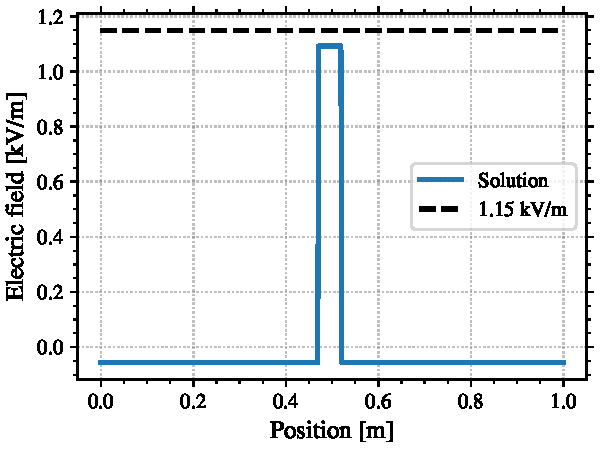
\includegraphics[width=\defaultwidth]{validation_dielectric_field.pdf}
      \caption{Electric field of the capacitor configuration calculated by the Poisson solver in order to validate the discretization and the solver developed. }
      \label{fig-surface}
    \end{figure}



  \subsection{Interface at the cell center}
    In the previous section, we supposed that the plasma-dielectric dielectric boundary was at the interface between the cells.
    However, this means that the electric field close to the interface is unknown, as it is defined at the cell center.
    Moreover, the Dirichlet condition for the potential is better defined at the cell center, and for the sake of simplicity, changing the boundary conditions should not change the particle domain.
    Hence, we chose to position the plasma-wall interface at the center of the cell as shown in \cref{fig-2D,fig-decompo2}.
    This means that the permittivity is not constant over a cell.

    Because the wall boundaries are only in the radial direction, we consider only an interface in the North-South direction.
    \Cref{fig-decompo2} shows the domain decomposition.
    The decomposition is the same as previously, except for the permittivity that can have two different values\string: one in the North half-plane ${\epsr}_{, i,j}^n$ and another in the South half plane ${\epsr}_{, i,j}^s$.

    \begin{figure}[hbt]
      \centering
      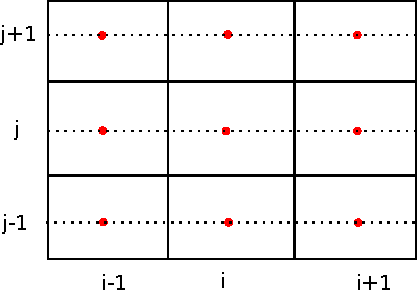
\includegraphics[width=\defaultwidth]{discrect2.pdf}
      \caption{Cartesian decomposition of the \acs{2D} domain. The dash lines represent discontinuities in the permittivity value.}
      \label{fig-decompo2}
    \end{figure}

    The discretization of the Poisson \cref{eq-poissonsum} follows the same path as previously, except that the electric flux in not constant anymore so that \cref{eq-poissonsum} becomes
    \begin{equation}
    \oint_{\C} (-\epsilon \grad \phi) \cdot \vect{n} dS = \sum_{k\in(E,W,N,S)} S^k_{i,j} <\vect{D}^k_{i,j} \cdot \vect{n}>.
    \end{equation}

    We can define
    \begin{align}
    <\vect{D}^E_{i,j} \cdot \vect{n} >&= \frac{1}{2} \epsilon_{i,j}^N E_{x, i+1/2,j}^- + \frac{1}{2} \epsilon_{i,j}^S E_{x, i+1/2,j}^-\\
     &= \frac{-1}{2} (\epsilon_{i,j}^N + \epsilon_{i,j}^S) \frac{\phi_{i+1/2,j} - \phi_{i,j}}{d_i/2}
     \label{eq-flux}
    \end{align}
    so that in the East-West direction, the flux behaves as if the cell permittivity is the mean of the North and South half-plane  $\epsilon_{i,j} = \frac{1}{2} (\epsilon_{i,j}^N + \epsilon_{i,j}^S)$.
    Hence, the rest of the computation is similar.
    For the boundary North and South, the permittivity is constant, hence there is no modification.
    Consequently, we obtain the discretization
    \begin{equation}
    S^E_{i,j} Q^E_{i,j} \phi_{i+1,j} + S^W_{i,j} Q^W_{i,j} \phi_{i-1,j} + S^N_{i,j} Q^N_{i,j} \phi_{i,j+1} + S^S_{i,j} Q^S_{i,j} \phi_{i,j-1} - Q^C_{i,j} \phi_{i,j} = - \V \bar{\rho_{i,j}}
    \label{eq-descretPoissoncentred}
    \end{equation}
    with
    \begin{center}
     $\begin{dcases}
     Q^E_{i,j} &= 2\frac{\epsilon_{i,j} \epsilon_{i+1,j}}{\epsilon_{i,j} d_{i+1} + \epsilon_{i+1,j} d_i} \\
     Q^W_{i,j} &= Q^E_{i-1,j} \\
     Q^N_{i,j} &= 2\frac{\epsilon_{i,j}^N \epsilon_{i,j+1}^S}{\epsilon_{i,j}^N d_{j+1} + \epsilon_{i,j+1}^S d_{j}}\\
     Q^S_{i,j} &= 2\frac{\epsilon_{i,j}^S \epsilon_{i,j-1}^N}{\epsilon_{i,j}^S d_{j+1} + \epsilon_{i,j-1}^N d_{j}} \\
     Q^C_{i,j} &= Q^E_{i,j}S^E_{i,j}+Q^W_{i,j}S^W_{i,j}+Q^N_{i,j}S^N_{i,j}+Q^S_{i,j}S^S_{i,j}
     \end{dcases}$
    \end{center}

    As well as $S^E_{i,j} = S^W_{i,j} =d_id_z, S^N_{i,j} = S^S_{i,j}= d_jd_z$ et $\V = d_jd_id_z$.
    Here, the system is no more symmetric.
    However, we can suppose that the only permittivity jump happens at the cell center, so that  $\epsilon_{i,j}^S = \epsilon_{i,j-1}^N$.
    Hence, $Q^N_{i,j} = 2\frac{\epsilon_{i,j}^N}{ d_{j+1} + d_{j}}$ and the system is symmetric.

  \subsection{Surface charges for centred interface}
    in the case of centred plasma-wall interface, we have surfaces charges at the center of the cell.
    Hence
    \begin{equation}
    \int_{\Omega_{i,j}} \rho dv = \Omega_{i,j}\bar{\rho} + S_{i,j}^N \sigma_{i,j}.
    \end{equation}
    The surface charges behave like volume charges.
    Hence, we obtain
    \begin{equation}
    S^E_{i,j} Q^E_{i,j} \phi_{i+1,j} + S^W_{i,j} Q^W_{i,j} \phi_{i-1,j} + S^N_{i,j} Q^N_{i,j} \phi_{i,j+1} + S^S_{i,j} Q^S_{i,j} \phi_{i,j-1} - Q^C_{i,j} \phi_{i,j} = - \V \bar{\rho_{i,j}} - S^N_{i,j} \sigma_{i,j}
    \end{equation}

    The discretization obtained for the plasma-wall interface cell-centred is very similar to the one obtained for the interface at the cell interface.
    However, it conserves the particle domain when the dielectric layer is not modeled, and that Dirichlet conditions are applied, and the electric field at the plasma-wall interface is better defined.
    Hence, the cell-centred interface will be used.

    \vspace{1em}
    This decomposition has been validate with the same test than presented in \cref{subsec-poisson_validation}.
    We observed no difference between the two decompositions in term of precision.
    
    
  \subsection{Electric field computation}
  
    The resolution of the Poisson equation returns the value of the plasma potential $\phi$ at the cell centers.
    The electric field is computed by taking the first derivative of the potential at the cell interface, as in \cref{eq-flux1},
    \begin{equation} \label{eq-E_ihalf}
      E_{x, i+1/2,j}^- = - \epsilon_{i,j} \frac{\phi_{i+1/2,j} - \phi_{i,j}}{d_i/2},
    \end{equation}
    with $\phi_{i+1/2,j}$ defined with \cref{eq-phidemi1}.
    However, in order to have consistent data, the electric field is also computed at the cell center by interpolation
    \begin{equation} \label{eq-E_mean}
      E_{x, i, j} = \frac{1}{2} \lp E_{x, i-1/2,j} + E_{x, i+1/2,j} \rp =  - \epsilon_{i,j} \frac{\phi_{i+1/2,j} - \phi_{i-i/2,j}}{d_i}.
    \end{equation}
    
    In the cells along to the plasma-wall interface, the effect of the surface charge must be taken into account, is previously described.
    
    \improvement{Can be more explicit here. Add exact expression of $E$ with $\phi_{i,j}$ and the effect of the surface charge.}
  
  
  
